\documentclass[]{beamer}
\usepackage{fancyvrb}
\usepackage{tikz}
\usetikzlibrary{arrows}
\tikzset{>=latex}

\newcommand{\myref}[1]{\small\item\url{#1}}
\newcommand{\myreff}[1]{\scriptsize\item\url{#1}}

\newcommand{\mthree}[9]{
\left[
\begin{array}{ccc}
#1 & #2 & #3 \\ #4 & #5 & #6 \\ #7 & #8 & #9
\end{array}
\right]
}

\newcommand{\mrowsix}[6]{
#1 & #2 & #3 & #4 & #5 & #6 
}

\newcommand{\bi}{\begin{itemize}}
\newcommand{\ei}{\end{itemize}}
\newcommand{\sect}[1]{
\section{#1}
\begin{frame}[fragile]\frametitle{#1}
}

\newcommand{\grph}[1]{
\begin{columns}
\column{0.01\textwidth}
\column{0.6\textwidth}
\includegraphics[scale=0.25]{figures/#1.png}
}


\newcommand{\txt}[1]{
\column{0.4\textwidth}
{\parbox{\textwidth}{
\small
\begin{itemize}
#1
\end{itemize}}}
\end{columns}}

\newcommand{\myvec}[1]{
\pstThreeDDot[showpoints=true,drawCoor=true](#1)
\pstThreeDLine[arrows=->,linecolor=blue](0,0,0)(#1)
}


\mode<presentation>
{
%  \usetheme{Madrid}
  % or ...

%  \setbeamercovered{transparent}
  % or whatever (possibly just delete it)
}

\usepackage[english]{babel}

\usepackage[latin1]{inputenc}

\title[Linear Algebra Notes I]
{
Linear Algebra Notes
}

%\subtitle{Based on Slides in MIT Open Courseware} % (optional)

\author[Geoffrey Matthews]
{Geoffrey Matthews}
% - Use the \inst{?} command only if the authors have different
%   affiliation.

\institute[WWU/CS]
{
  Department of Computer Science\\
  Western Washington University
}
% - Use the \inst command only if there are several affiliations.
% - Keep it simple, no one is interested in your street address.

\date{Fall 2011}

% If you have a file called "university-logo-filename.xxx", where xxx
% is a graphic format that can be processed by latex or pdflatex,
% resp., then you can add a logo as follows:

%\pgfdeclareimage[height=0.5cm]{university-logo}{WWULogoProColor}
%\logo{\pgfuseimage{university-logo}}

% If you wish to uncover everything in a step-wise fashion, uncomment
% the following command: 

%\beamerdefaultoverlayspecification{<+->}
\newcommand{\point}[2]{
  \fill (#1) node (#2) {} circle (2pt) node[anchor=south] {$#2$};
  }
\newcommand{\pointn}[2]{
  \fill (#1) node (#2) {} circle (2pt) node[anchor=north] {$#2$};
  }
\newcommand{\coords}{
      \draw[dotted,step=1] (0,0) grid (9.9,9.9);
      \draw[thick,<->] (10,0) %node[anchor=west] {$x$ axis}
      -- (0,0) -- (0,10) %node[anchor=south] {$y$ axis}
      ;
      \foreach \x in {0,1,2,3,4,5,6,7,8,9}
        \draw (\x ,2pt) -- (\x ,-2pt) node[anchor=north] {$\x$};
      \foreach \y in {0,1,2,3,4,5,6,7,8,9}
        \draw (2pt,\y) -- (-2pt,\y ) node[anchor=east] {$\y$};
}

\begin{document}


\begin{frame}
  \titlepage
\end{frame}

%\begin{frame}
%  \frametitle{Outline}
%  \tableofcontents
%  % You might wish to add the option [pausesections]
%\end{frame}


\sect{Online Resources}

{\bf Readings}
\begin{itemize}
  \myref{http://chortle.ccsu.edu/vectorlessons/vectorindex.html}
  \myref{http://mathforum.org/mathimages/index.php/Math_for_Computer_Graphics_and_Computer_Vision}
\myref{http://cs229.stanford.edu/section/cs229-linalg.pdf}

\myreff{http://ocw.mit.edu/courses/electrical-engineering-and-computer-science/}, Computer graphics
\myref{http://joshua.smcvt.edu/linearalgebra/}
\end{itemize}
{\bf Videos}
\begin{itemize}
\myref{http://www.khanacademy.org/math/linear-algebra}
\end{itemize}
\end{frame}

\sect{Matrices}
\begin{itemize}
\item A matrix is a set of scalars organized into rows and columns.
\end{itemize}
\[
\left[\begin{array}{cc}
a & b \\
c & d \\
\end{array}
\right]
\]

\end{frame}

\sect{Matrix addition, subtraction, multiplication}
\begin{eqnarray*}
\left[\begin{array}{cc}
a & b \\
c & d \\
\end{array}
\right]
+
\left[\begin{array}{cc}
e & f \\
g & h \\
\end{array}
\right]
&=&\left[\begin{array}{cc}
a+e & b+f \\
c+g & d+h \\
\end{array}
\right]\\
\left[\begin{array}{cc}
a & b \\
c & d \\
\end{array}
\right]
-
\left[\begin{array}{cc}
e & f \\
g & h \\
\end{array}
\right]
&=&\left[\begin{array}{cc}
a-e & b-f \\
c-g & d-h \\
\end{array}
\right]\\
\left[\begin{array}{cc}
a & b \\
c & d \\
\end{array}
\right]
\left[\begin{array}{cc}
e & f \\
g & h \\
\end{array}
\right]
&=&\left[\begin{array}{cc}
ae+bg & af+bh \\
ce+dg & cf+dh \\
\end{array}
\right]
\end{eqnarray*}
\end{frame}

\sect{Multiplication is {\em not} commutative!  $MN \not=NM$}
\begin{eqnarray*}
\left[\begin{array}{cc}
a & b \\
c & d \\
\end{array}
\right]
\left[\begin{array}{cc}
e & f \\
g & h \\
\end{array}
\right]
&=&\left[\begin{array}{cc}
ae+bg & ... \\
... & ... \\
\end{array}
\right]
\\
\left[\begin{array}{cc}
e & f \\
g & h \\
\end{array}
\right]
\left[\begin{array}{cc}
a & b \\
c & d \\
\end{array}
\right]
&=&\left[\begin{array}{cc}
ea+fc & ... \\
... & ... \\
\end{array}
\right]
\end{eqnarray*}
\end{frame}

\sect{Mathematical Vectors}
\begin{eqnarray*}
\vec{v} &=& \left[\begin{array}{c} a\\b\\c \end{array}\right]\\
        &=& [a\  b\  c]^T \\
        &=& (a,b,c)
\end{eqnarray*}
\begin{itemize}
\item A vector is an $N$ row by 1 column matrix.
\item We will use mathematical vectors to represent both {\em points} and {\em vectors} in space.
\end{itemize}
\end{frame}

\sect{Matrices as transforms}
\begin{itemize}
\item{Multiplication of an $N$-vector by an $N\times N$ matrix {\em on the
  left} changes it into another $N$-vector.}
\end{itemize}
\[
\left[\begin{array}{ccc}a&b&c\\d&e&f\\g&h&i\end{array}\right]
\left[\begin{array}{c}x\\y\\z\end{array}\right]
=
\left[\begin{array}{c}x'\\y'\\z'\end{array}\right]
\]
\end{frame}

\sect{Matrix inverses}
\begin{itemize}
\item Identity matrix: \[I=\left[\begin{array}{ccc}1&0&0\\0&1&0\\0&0&1\end{array}\right]\]
\item $AI = IA = A$
\item Some matrices have an inverse: $AA^{-1} = A^{-1}A = I$
\item $(ABC)^{-1} = C^{-1}B^{-1}A^{-1}$
\end{itemize}

\end{frame}

\sect{Determinant of a matrix}
\begin{eqnarray*}
A &=& \left[\begin{array}{cc}
a & b \\
c & d \\
\end{array}\right]\\
\mbox{det}(A) &=&  \left|\begin{array}{cc}
a & b \\
c & d \\
\end{array}\right|\\
&=& ad-bc\\
A^{-1} &=& \frac{\left[\begin{array}{cc}d&-b\\-c&a\end{array}\right]}{\mbox{det}(A)}
\end{eqnarray*}
\end{frame}

\sect{Determinant of a matrix}
\begin{eqnarray*}
\left|\begin{array}{ccc}a&b&c\\d&e&f\\g&h&i\end{array}\right|
&=&
a\left|\begin{array}{cc}e&f\\h&i\end{array}\right|
-b\left|\begin{array}{cc}d&f\\g&i\end{array}\right|
+c\left|\begin{array}{cc}d&e\\g&h\end{array}\right|\\
&=& (aei - afh) - (bdi - bfg) + (cdh - ceg)\\
&=& aei + bfg + cdh - afh - bdi - ceg
\end{eqnarray*}
\end{frame}

\sect{Cross product (vector product)}
\begin{columns}
  \begin{column}{0.6\textwidth}
    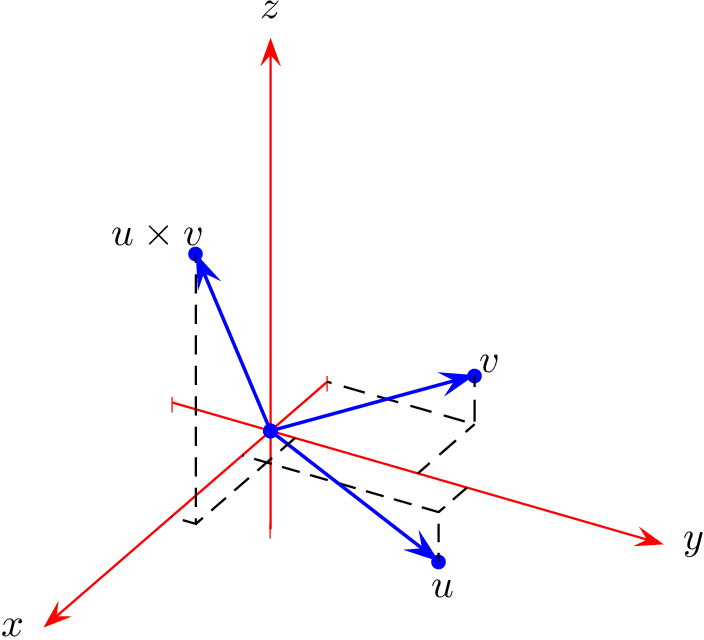
\includegraphics[scale=0.25]{figures/crossprod.png}
  \end{column}
  \begin{column}{0.4\textwidth}
    \begin{itemize}
    \item A vector at right angles to $u$ and $v$.
    \item $u \times v = $\\
      $(u_2v_3 - u_3v_2,$\\$ u_3v_1 - u_1v_3,$\\$ u_1v_2 - u_2v_1)$
      
    \item Mnemonic:
      \[u\times v = \left|\begin{array}{ccc}
      \vec{i} & \vec{j} & \vec{k} \\
      u_1 & u_2 & u_3 \\
      v_1 & v_2 & v_3 \\
      \end{array}\right|\]
    \item $|u\times v| = |u||v|\sin(\theta)$
    \end{itemize}
  \end{column}
\end{columns}

\end{frame}

\sect{Inverse of a matrix}
\[
\left[\begin{array}{cccccc}a&b&c&1&0&0\\
d&e&f&0&1&0\\
g&h&i&0&0&1\end{array}\right]
\]
\begin{itemize}
\item Stick the identity on the right.
\item Add multiples of one row to another until the identity is on the left.
\item The inverse is now on the right
\end{itemize}
\end{frame}


\end{document}
